\documentclass[]{article}


\usepackage[preprint]{neurips_2020}
\usepackage[T1]{fontenc}    
\usepackage{hyperref}       
\usepackage{url}            
\usepackage{booktabs}       
\usepackage{amsfonts}       
\usepackage{nicefrac}       
\usepackage{microtype}      
\usepackage[shortlabels]{enumitem}
\usepackage{amsmath}
\usepackage{amssymb}
\usepackage{xeCJK}
\usepackage{color}
\usepackage{graphicx}


\setCJKmainfont{微軟正黑體}
\hypersetup{
	colorlinks   = true, 
	urlcolor     = blue, 
	linkcolor    = blue, 
	citecolor    = red 
}


\title{CUDA驅動蟻群模擬器}
\author{
	鄭適其\\
	309612092 \\
	土木工程學系\\
	國立陽明交通大學 \\
}

\begin{document}

\maketitle
\tableofcontents

\clearpage
\section{簡介}
\label{intro}
\paragraph{}
在夏天的戶外,我們常常可以看見螞蟻們成群結隊、井然有序地把食物搬到牠們的巢穴中,不禁讓人感嘆大自然的奧妙。但是我卻也非常好奇這些小小的螞蟻怎麼會有如此的智慧,在查過資料後,大概了解了螞蟻是依靠在走過的路上留下特殊的費洛蒙,來指引同伴食物或巢穴的位置,並藉由控制留下費洛蒙的量以及運用費洛蒙會揮發的特性,構建出一條往返食物與巢穴的橋樑。
\paragraph{}
本專案就是要透過Python中的Tkinter視窗套件視覺化這樣生物的機制,並且在這之中使用CUDA平行運算來加速取得人工螞蟻們的行徑方向。不過計算速度在Python中仍然是短版,因此本專案對真實的螞蟻仍然做了簡化,並非完整的螞蟻找食物機制,但是可以確保人工螞蟻們能在自訂義的2D地圖上找到往返食物與巢穴的路。


\section{演算法細節}
\label{algo}

\subsection{定義}
\label{algo:cls}
\paragraph{}
人工螞蟻(以下簡稱\textbf{螞蟻})有分成兩種狀態:
\begin{enumerate}[(a)]
	\item \textbf{尋找食物狀態}(\textbf{Look at Food}, \textbf{LF}),即未找到食物的螞蟻。
	\item \textbf{尋找巢穴狀態}(\textbf{Look at Home}, \textbf{LH}),即已找到食物的螞蟻。
\end{enumerate}
\paragraph{}
費洛蒙也分成兩種:
\begin{enumerate}[(a)]
	\item \textbf{指引食物}(\textbf{Guide to Food}, \textbf{GF})
	\item \textbf{指引巢穴}(\textbf{Guide to Home}, \textbf{GH})
\end{enumerate}
\paragraph{}
其他定義:
\begin{itemize}
	\item \textbf{速度}: \ 包含移動\textbf{距離}與\textbf{方向}。
\end{itemize}
\paragraph{}
重點目標: \ \textcolor{red}{LF的目標是不斷找尋一定範圍內最大GF所在的方向,而LH則是不斷尋找一定範圍內最大GH所在的方向}。

\subsection{世界更新方式}
\label{algo:world}
\subsubsection{生成移動場}
\label{algo:world:field}
\paragraph{}
在螞蟻們移動前,會依照地圖上殘留的費洛蒙來生成每個位置(像素)對應的最大費洛蒙方向,這個動作是由CUDA平行運算完成,這也是驅動整個蟻群移動的 \textcolor{blue}{\textbf{核心引擎}}。每個位置對應到一組長度為3的向量,各元素對應的意義為:
\begin{equation}\label{algo:world:field:vector}
	[\texttt{是否附近所有值皆相等}, \texttt{最大值所在}X, \texttt{最大值所在}Y]
\end{equation}
\paragraph{}
第一個值若是True,則在那個位置上的螞蟻會隨機移動。而自身位置不會被列入考慮,避免可能出現螞蟻不會移動的情況。另外,地圖邊界外、牆壁內的位置也不考慮。
\subsubsection{費洛蒙殘留}
\label{algo:world:pheromRes}
\paragraph{}
每隻螞蟻每次移動時都會留下費洛蒙,LF會留下GH,LH會留下GF。而每走一步留下的費洛蒙會越來越少,這麼做的目的是為了使越接近食物或巢穴的地方,費洛蒙殘留量越高。所以螞蟻向著費洛蒙愈大的地方走,就可以解釋成離食物或巢穴愈接近。
\subsubsection{費洛蒙揮發}
\label{algo:world:pheromEvap}
\paragraph{}
每次iteration都會讓地圖上的費洛蒙揮發一些,是蟻群能找到最佳的路徑的關鍵。因為根據\ref{algo:world:pheromRes}可知,路徑長度愈長,費洛蒙補充的越少,因此若已知地圖每個位置的揮發率相同,則長度較長的路徑會越容易消失,而較短路徑會留下。

\subsection{移動方式}
\label{algo:move}
\paragraph{}
最主要的走法還是要瞄準相對目前位置的一定範圍內最大費洛蒙方向(為了簡化計算,此範圍是正方形),但是單純的這麼做會遇到一些問題。
\subsubsection{區域極值問題}
\label{algo:move:localmax}
\paragraph{}
首先是最佳化中最惡名昭彰的問題: \textbf{Local Maximum} 與 \textbf{Local Minimum},而因為螞蟻的目標是找最大值,所以只有local maximum問題。因此本專案參考了深度學習中optimizer常用的技巧 \textbf{momentum},也就是藉由將上個iteration的速度與本次iteration的速度做線性組合做為新的速度在本次iteration中使用(如eq\eqref{algo:move:localmax:momentum}所示)。從實驗的結果看來,momentum確實能有效使螞蟻脫離local maximum。
\begin{equation}\label{algo:move:localmax:momentum}
	v'_{t}(s_{t}) \leftarrow \alpha \cdot v_{t-1}(s_{t-1}) + (1 - \alpha) \cdot v_{t}(s_{t}) \ , \ 0 \leq \alpha \leq 1
\end{equation}
\paragraph{}
$v$是速度,$\alpha$是權重,$s$是位置向量,$t$是迭代次數。另外,食物與巢穴位置是global maximum,因為在此專案中,假設它們的費洛蒙值始終維持無窮大,讓到它們附近的螞蟻可以被快速吸引過去。
\subsubsection{邊界問題}
\label{algo:move:boundary}
\paragraph{}
由於Tkinter的Canvas範圍是有限的,而我們不能螞蟻走出邊界,另外為了檢驗演算法的效果,本專案設計了可以在地圖上加上牆壁的機制,而螞蟻不能穿過牆壁。也就是說,螞蟻們是不能隨便走動的,因此所有的螞蟻都具有碰牆反彈的機制。但有得時候螞蟻仍然會走出界或是走到牆壁裡,因此在走之前要檢查sample到的速度是否會走出界或進到牆壁,如果有那就讓螞蟻在這個iteration靜止不動,但是保留一半的速度作為momentum。
\subsubsection{缺乏探索問題}
\label{algo:move:exploration}
\paragraph{}
為了增強蟻群的探索(exploration),螞蟻的每次行動都有隨機性,也就是螞蟻會有一定的機率不按照最大費洛蒙方向走。如果所有螞蟻只會按照現有的路線走,那就無法找到路徑更短的新路線以加快食物取得速度,因此行動的隨機性是相當重要的。另外,經由實驗發現momentum也有增強蟻群探索速度的效果。故移動速度的期望值可寫成:
\begin{equation}\label{algo:move:exploration:moveExpect}
	\mathbb{E}_p\{v_{t}(s_{t})\} \stackrel{def}{=} (1 - p) \cdot v'_{t}(s_{t}) + p \cdot \mathbf{Clip} (Random \ Vector, -speed, speed)
\end{equation}
\paragraph{}
其中$p$為隨機移動機率,$speed$是移動距離。
\subsubsection{LH和LF的差異}
\paragraph{}
為了加速LF找到食物,LF在GF的向量\eqref{algo:world:field:vector}第一個元素為True時,會採取GH最大值方向的反向($ -\mathbb{E}^{GH}_{\textcolor{red}{(1-p)}}\{v_{t}(s_{t})\} $)作為移動目標,當附近有出現GF時就改用$ \mathbb{E}^{GF}_p\{v_{t}(s_{t})\} $。而LH沒有相對應的機制,依然只依靠$ \mathbb{E}^{GH}_p\{v_{t}(s_{t})\} $作為移動依據。

\subsection{蟻群自我調節方式}
\label{algo:colony}
\subsubsection{螞蟻的出生}
\label{algo:colony:born}
\paragraph{}
當收集到的食物達到足夠的量,則可以新出生更多螞蟻擴大蟻群,可以及時補充地圖上的費洛蒙,使蟻群可以找到更遠的食物,或是更加鞏固現有的道路。
\subsubsection{螞蟻的死亡}
\label{algo:colony:death}
\paragraph{}
當LF太久沒有找到食物,則會有機率餓死。因為食物量不變,每餓死一隻螞蟻就會有一隻新螞蟻在巢穴出生。可以重新補充地圖的費洛蒙。
\subsubsection{螞蟻吃掉食物}
\label{algo:colony:eatFood}
\paragraph{}
當LH太久沒找到巢穴,則他會把食物吃掉以存活,並且將狀態從LH轉成LF,並在找到新食物前不會再留下任何費洛蒙。

\clearpage
\section{GUI介面}
\label{interface}
\begin{figure}[htbp]
	\centering
	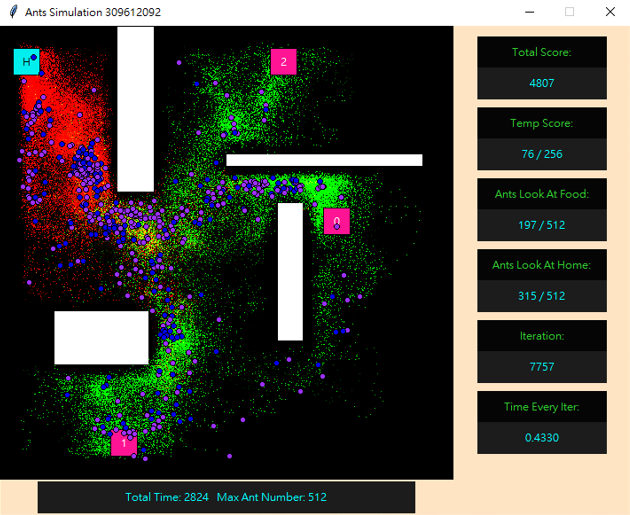
\includegraphics[width=1.0\linewidth]{../interface}
	\caption{GUI介面}
	\label{interface:fig}
\end{figure}
\paragraph{}
如Figure \ref{interface:fig}所示,程式實際執行起來會出現這樣的GUI介面:
\begin{itemize}
	\item \textbf{右方面板}:
	\subitem \textbf{Total Score}: 總得分(每帶一單位食物回巢得一分)
	\subitem \textbf{Temp Score}: 暫時得分,當累積到總螞蟻數的一半會產生一群新螞蟻,並且分數歸零
	\subitem \textbf{Ants Look At Food}: 有多少螞蟻處於LF狀態
	\subitem \textbf{Ants Look At Home}: 有多少螞蟻處於LH狀態
	\subitem \textbf{Iteration}: 目前迭代次數
	\subitem \textbf{Time Every Iter}: 每次迭代所需時間
	
	\item \textbf{下方面板}:
	\subitem \textbf{Total Time}: 總經過時間
	\subitem \textbf{Max Ant Number}: 最大螞蟻數量
	
	\item \textbf{中間面板}:
	\subitem \textbf{藍點}: LF
	\subitem \textbf{綠點}: LH
	\subitem \textbf{白色}: 牆壁
	\subitem \textbf{紅點}: GH
	\subitem \textbf{綠點}: GF
	\subitem \textbf{水藍色正方形}: 螞蟻巢穴
	\subitem \textbf{粉紅色正方形}: 食物
\end{itemize}


\section{實驗記錄}
\label{experiment}

\subsection{地圖0}
\begin{figure}[htbp]
	\centering
	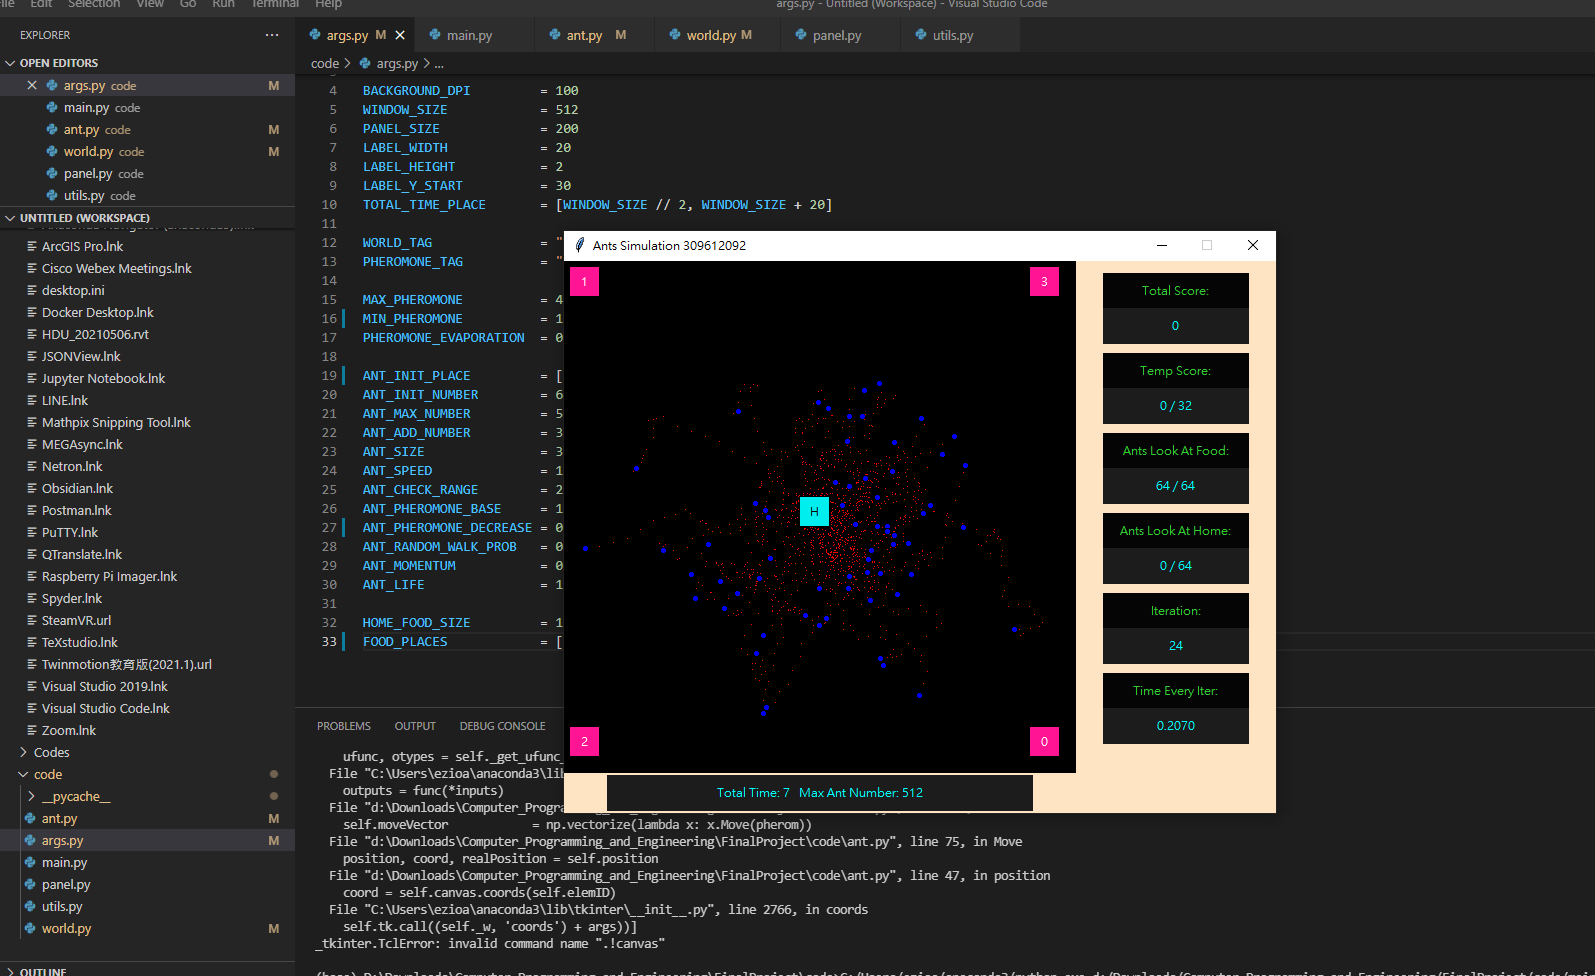
\includegraphics[width=0.9\linewidth]{../record8}
	\label{fig:record8}
\end{figure}
\begin{figure}[htbp]
	\centering
	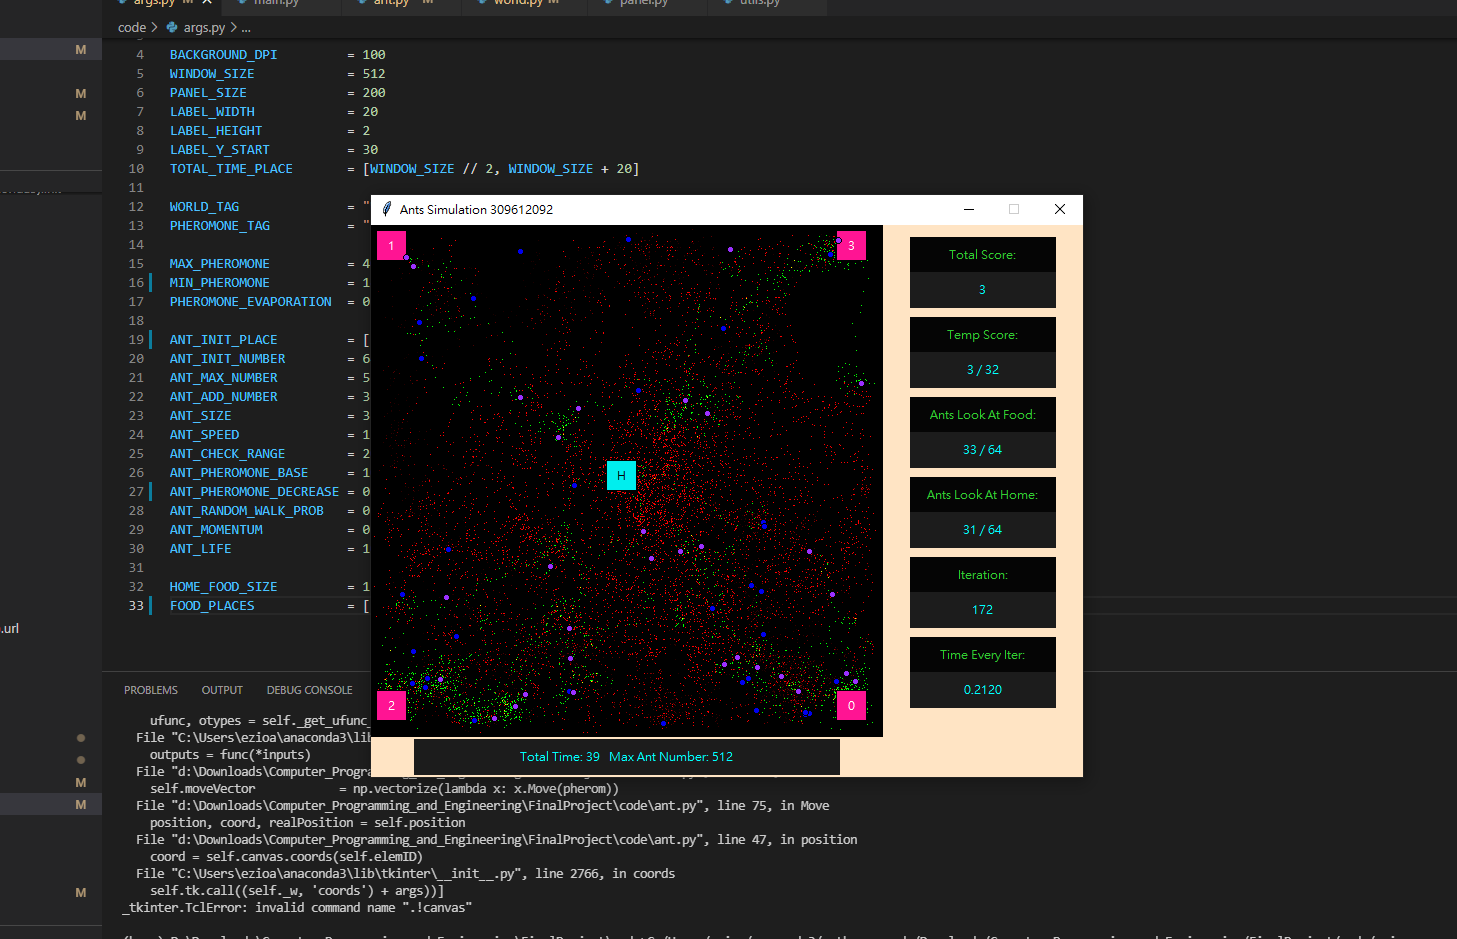
\includegraphics[width=0.9\linewidth]{../record9}
	\label{fig:record9}
\end{figure}
\begin{figure}[htbp]
	\centering
	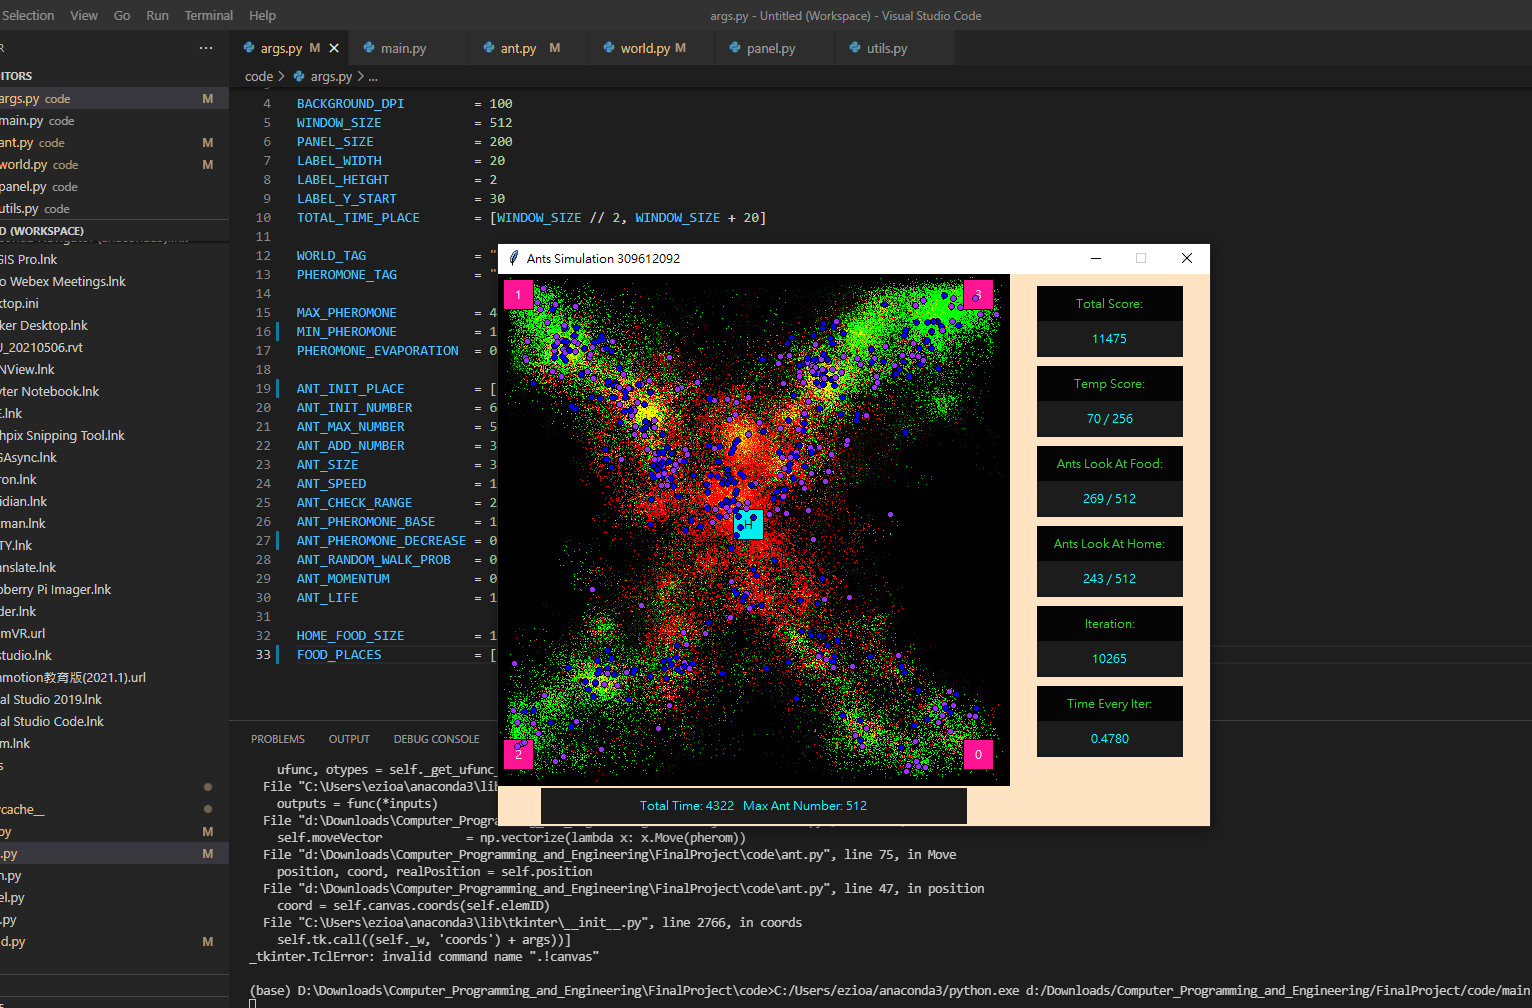
\includegraphics[width=0.9\linewidth]{../record10}
	\label{fig:record10}
\end{figure}

\clearpage
\subsection{地圖1}
\begin{figure}[htbp]
	\centering
	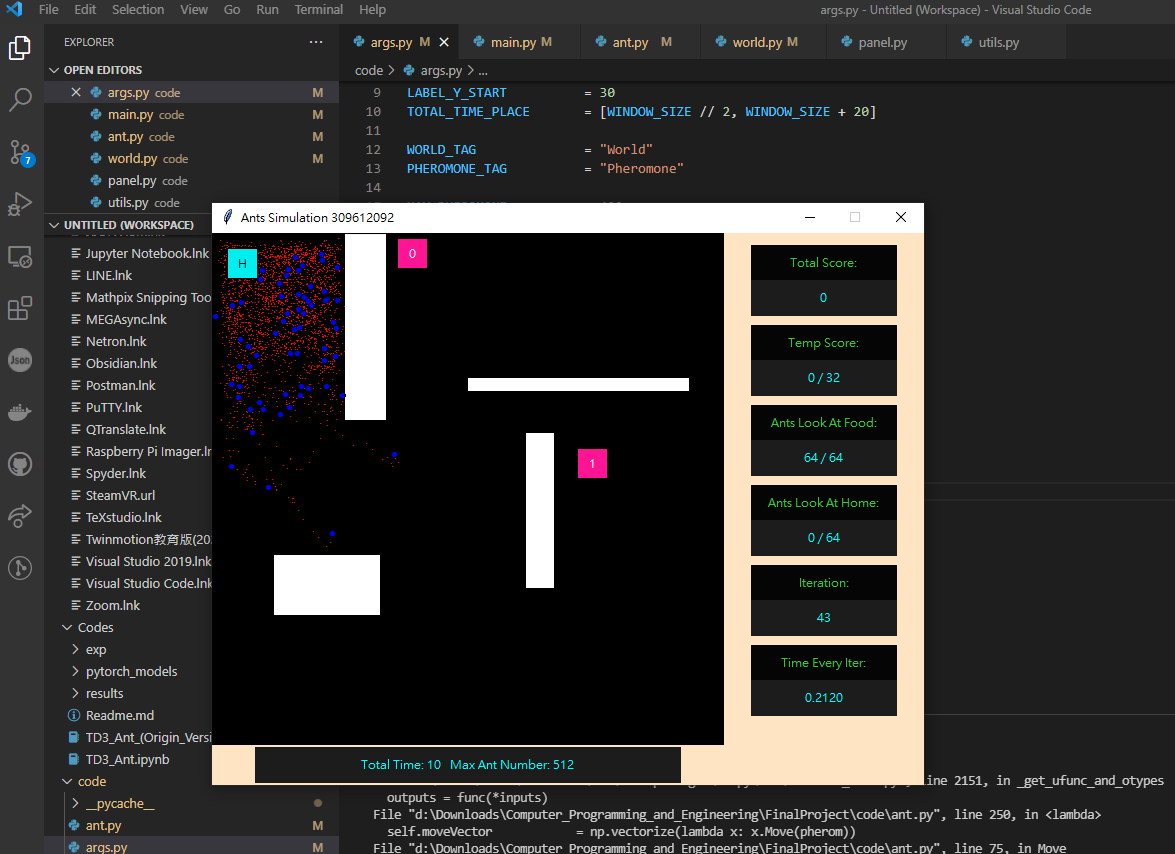
\includegraphics[width=0.9\linewidth]{../record1}
	\label{fig:record1}
\end{figure}
\begin{figure}[htbp]
	\centering
	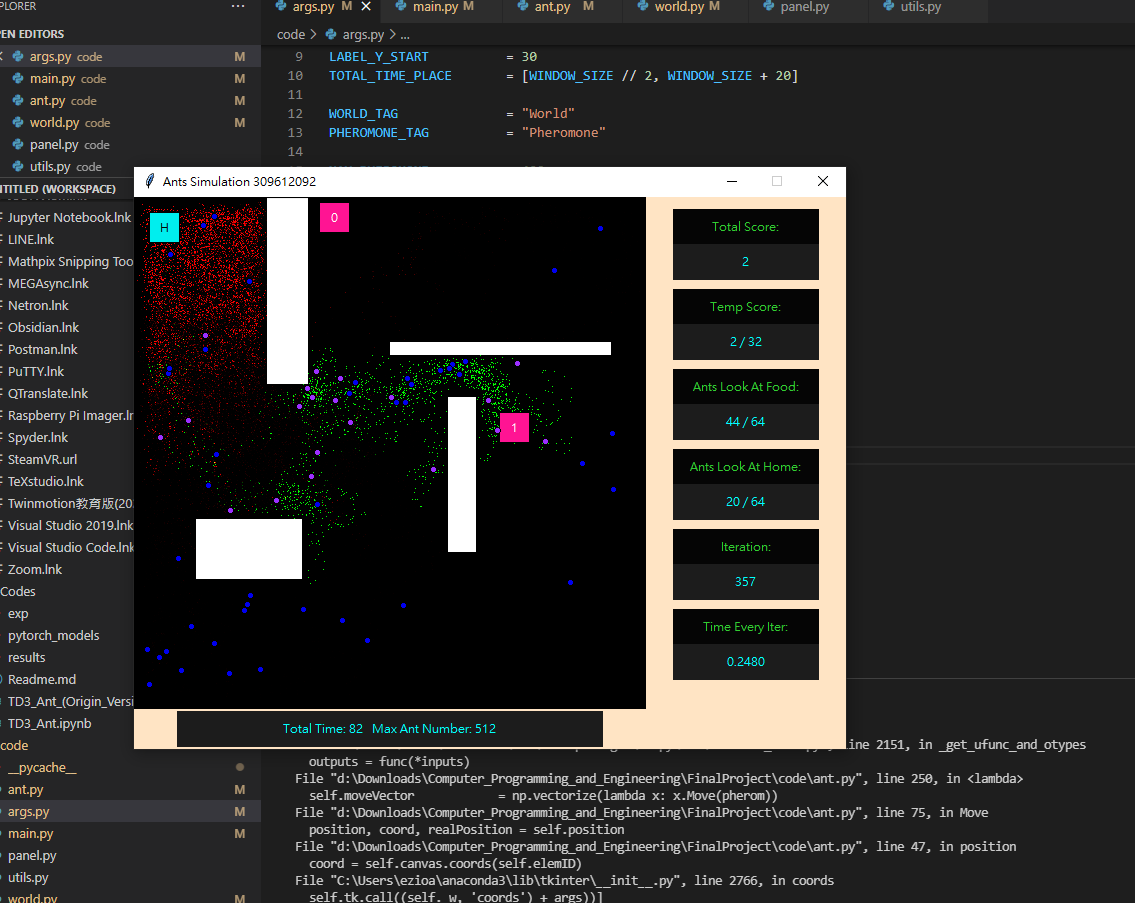
\includegraphics[width=0.9\linewidth]{../record2}
	\label{fig:record2}
\end{figure}
\begin{figure}[htbp]
	\centering
	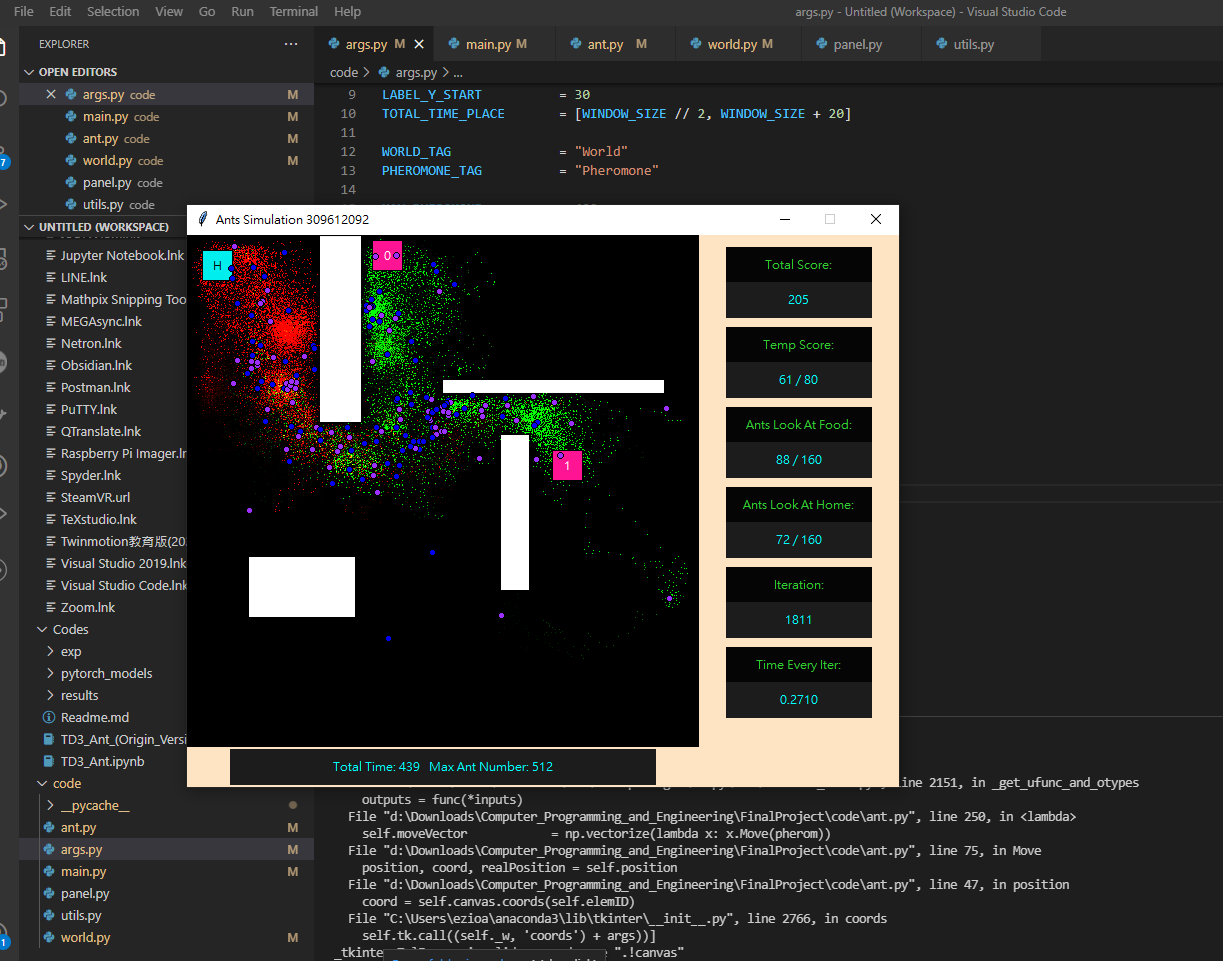
\includegraphics[width=0.9\linewidth]{../record3}
	\label{fig:record3}
\end{figure}
\begin{figure}[htbp]
	\centering
	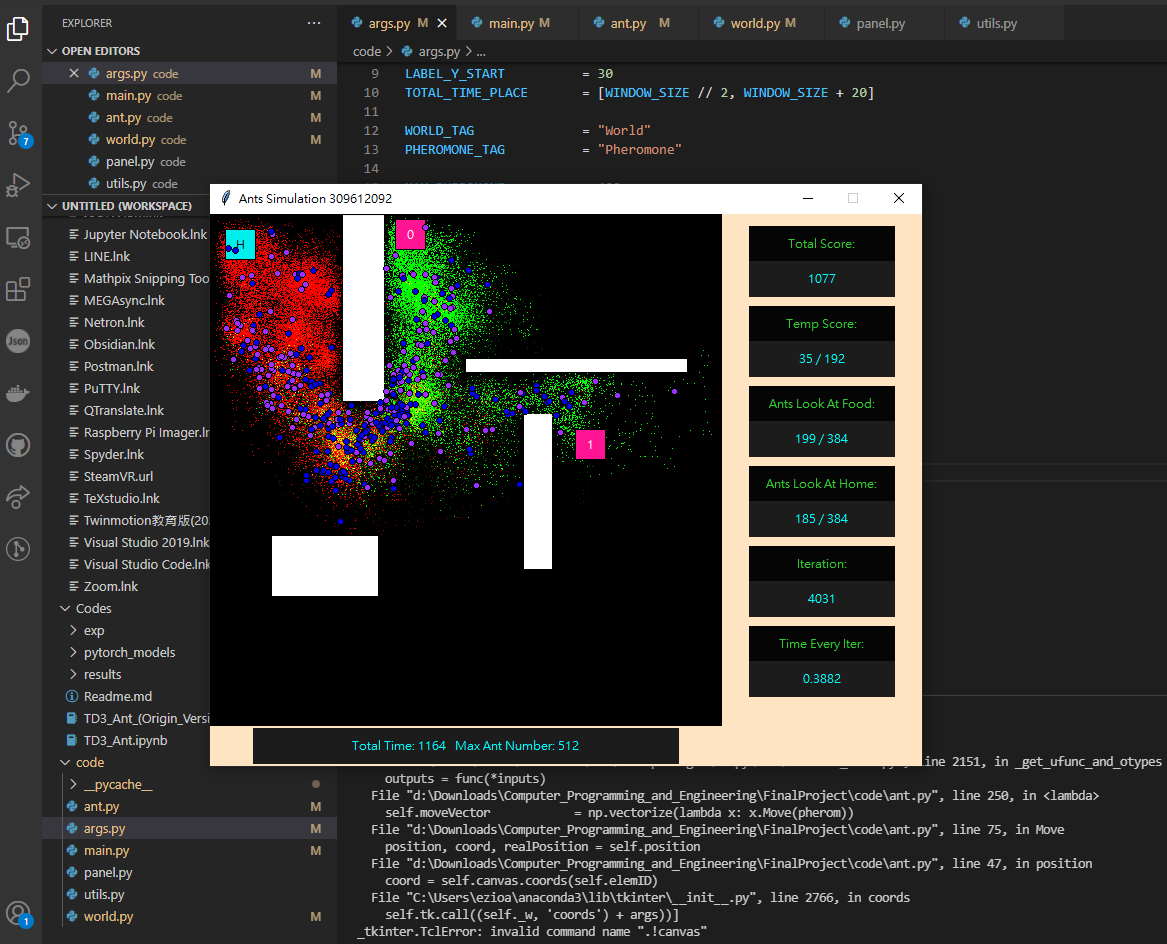
\includegraphics[width=0.9\linewidth]{../record4}
	\label{fig:record4}
\end{figure}

\clearpage
\subsection{地圖2}
\begin{figure}[htbp]
	\centering
	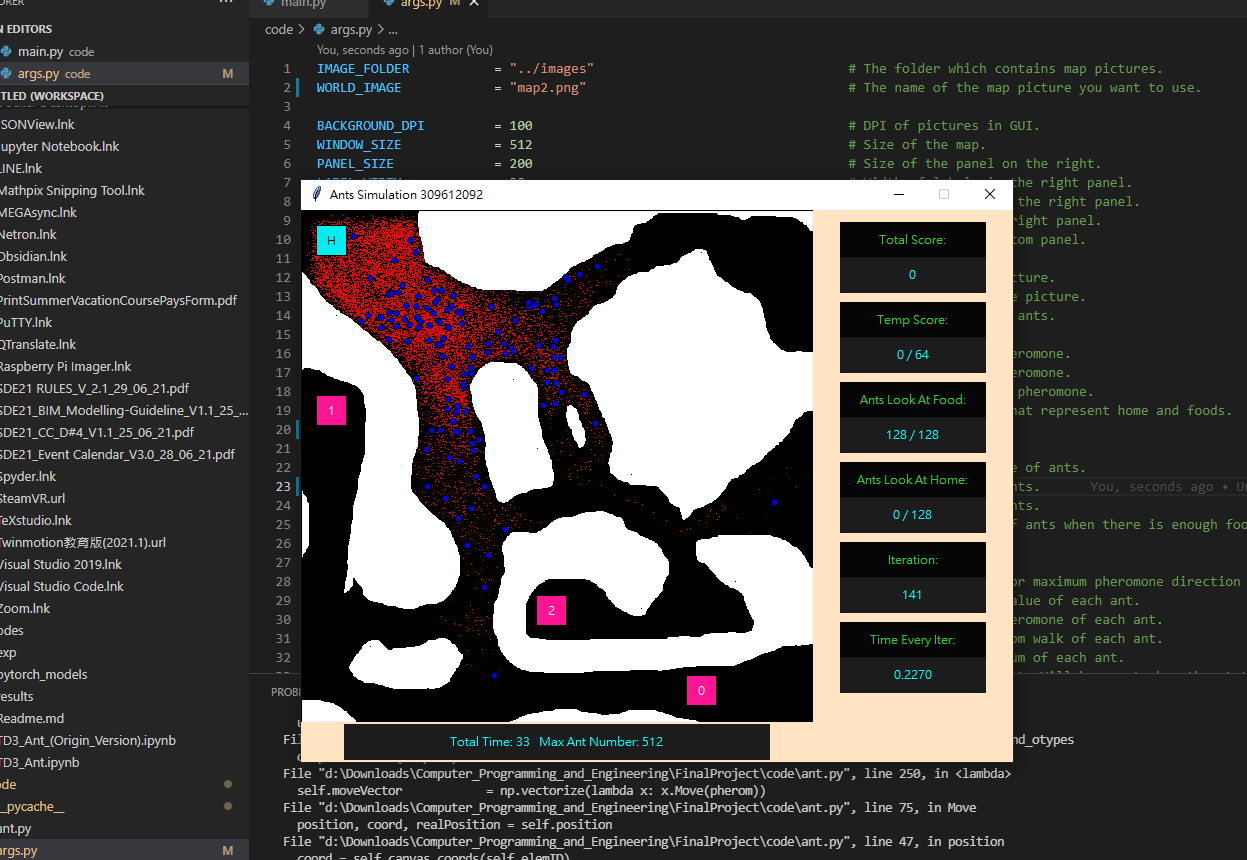
\includegraphics[width=0.9\linewidth]{../record5}
	\label{fig:record5}
\end{figure}
\begin{figure}[htbp]
	\centering
	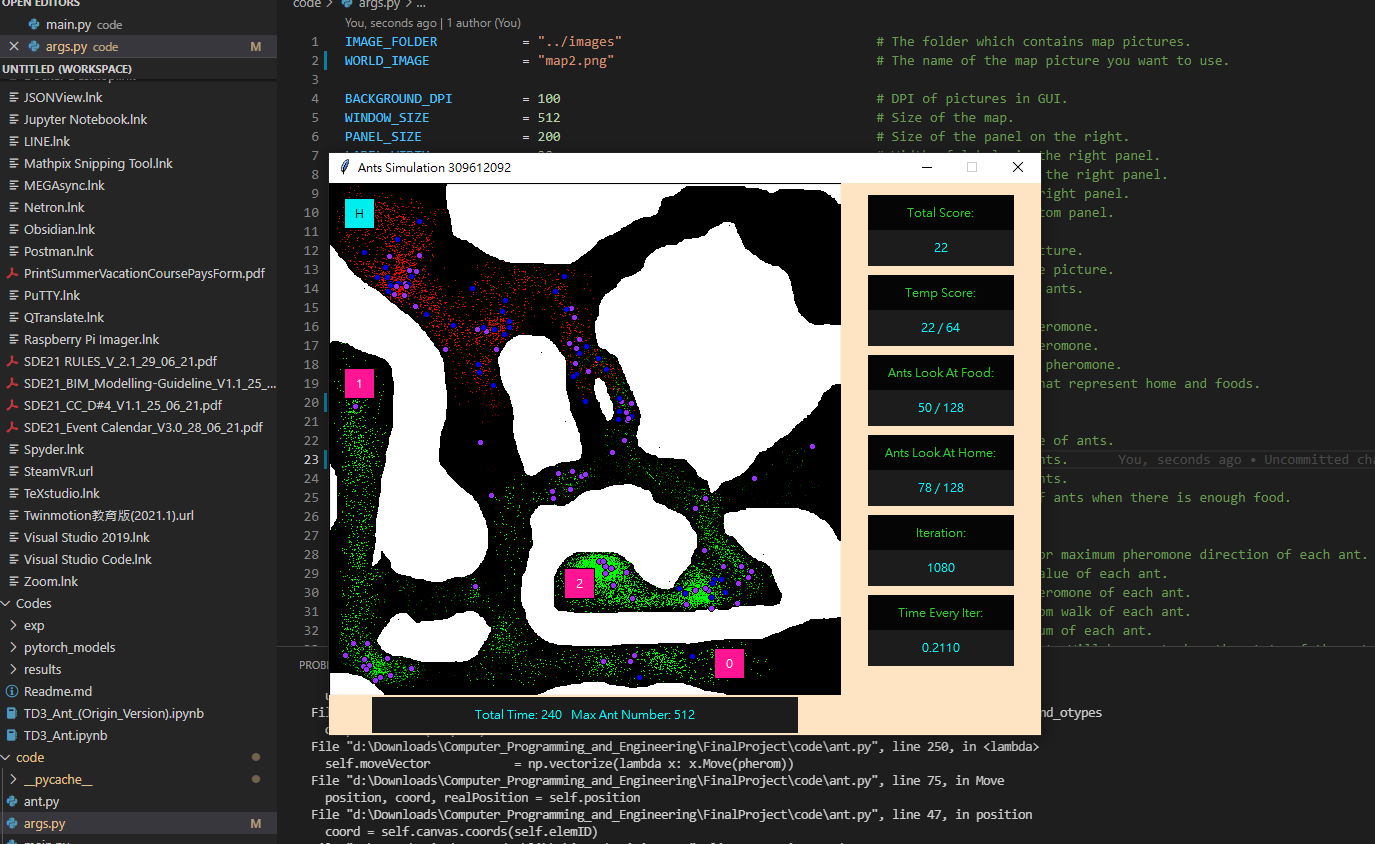
\includegraphics[width=0.9\linewidth]{../record6}
	\label{fig:record6}
\end{figure}
\begin{figure}[htbp]
	\centering
	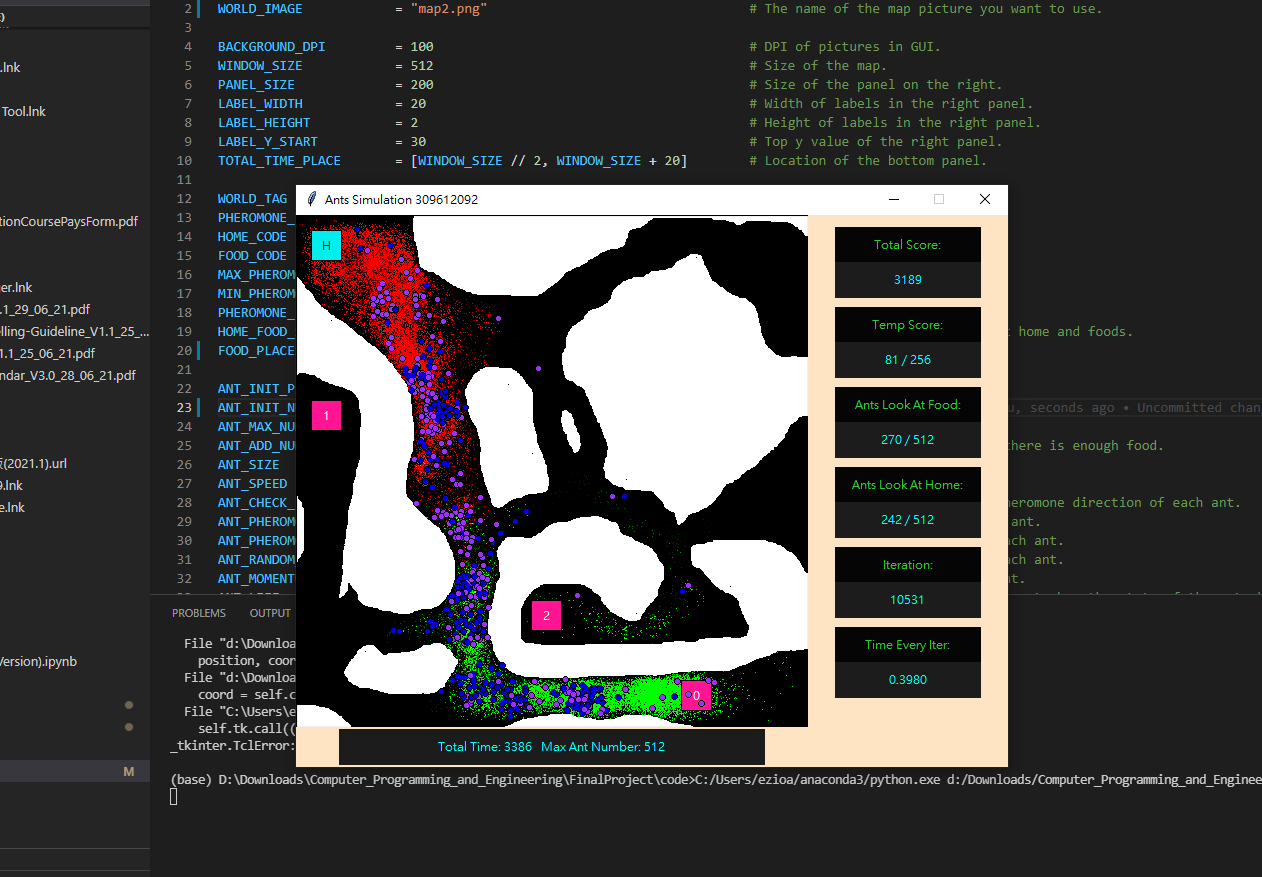
\includegraphics[width=0.9\linewidth]{../record7}
	\label{fig:record7}
\end{figure}


\clearpage
\section{程式碼}

\subsection{程式簡介}
\paragraph{}
程式檔案用途:
\begin{itemize}
	\item \textbf{args.py}: 參數設置
	\item \textbf{main.py}: 主程式循環
	\item \textbf{ant.py}: 螞蟻、蟻群相關程式碼
	\item \textbf{world.py}: 世界、費洛蒙地圖相關程式碼
	\item \textbf{panel.py}: GUI右方與下方panel相關程式碼
	\item \textbf{utils.py}: 雜項
\end{itemize}
\paragraph{}
自訂義6大class介紹:
\begin{itemize}
	\item \textbf{BG\_Manager}: 背景管理(World與PheromoneMap的父類別)
	\item \textbf{World}: 世界地圖
	\item \textbf{PheromoneMap}: 費洛蒙地圖
	\item \textbf{Ant}: 人工螞蟻
	\item \textbf{AntColony}: 蟻群統籌管理
	\item \textbf{Panel}: GUI右方與下方儀表板
\end{itemize}

\subsection{使用方式}
\begin{enumerate}[(a)]
	\item 在args.py中調整參數(參數意義寫在程式碼註解中)。
	\item 調整參數後執行main.py。
	\item 彈出Tkinter的視窗即執行成功。
\end{enumerate}
\paragraph{}
若要自行設計地圖,請注意地圖只能是二值圖片(即只有黑色與白色),白色部分會被當作牆壁,黑色部分為螞蟻可走範圍,此設定無法由參數更改。由於簡化計算之故,盡量不要把牆壁畫得太薄,厚度至少大於args.py裡的ANT\_SPEED(單位: pixel),否則螞蟻可能會穿牆。最後記得要調整args.py中的FOOD\_PLACES(食物位置,可有多個)以及ANT\_INIT\_PLACE(螞蟻巢穴位置,只能有一個)。

\end{document}


